\subsection{Observer}
Viene utilizzato per stabilire una relazione 1 a n tra un oggetto e altri vari oggetti che dipendo da esso.
Ogni volta che l'oggetto osservato viene modificato, questo si preoccupa di comunicarlo agli oggetti che lo osservano.

\begin{figure}[ht]
    \centering
    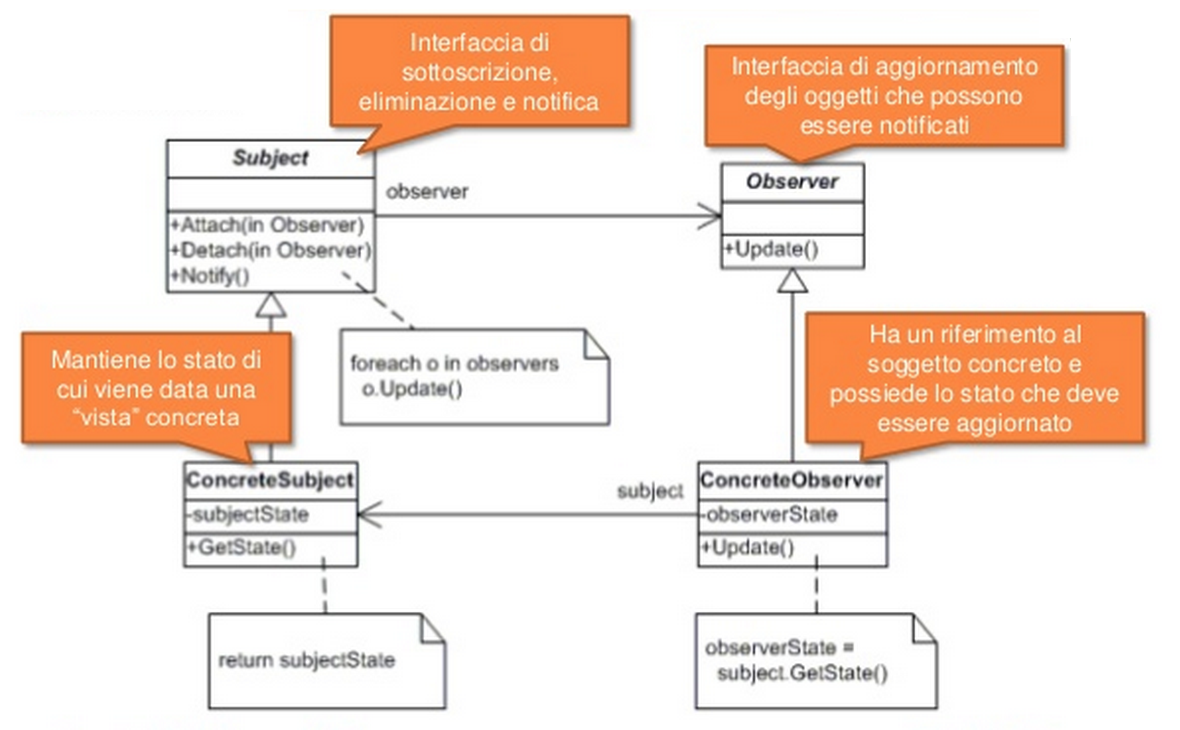
\includegraphics[width=0.8\textwidth]{immagini/observer.png}
    \caption{Proxy}
\end{figure}
\FloatBarrier

Possono essere fatte versioni più smart, dove l'oggetto osservato comunica anche che cosa è stato modificato oppure avverte solo alcuni oggetti registrati, in modo da evitare chiamate a funzioni inutili.

\subsubsection{Utilizzo}
\begin{enumerate}
\item Il soggetto viene modificato;
\item Il soggetto notifica tutti gli osservatori registrati;
\item I vari osservatori si sincronizzano sui cambiamenti subiti dal soggetto.
\end{enumerate}
\begin{figure}[ht]
    \centering
    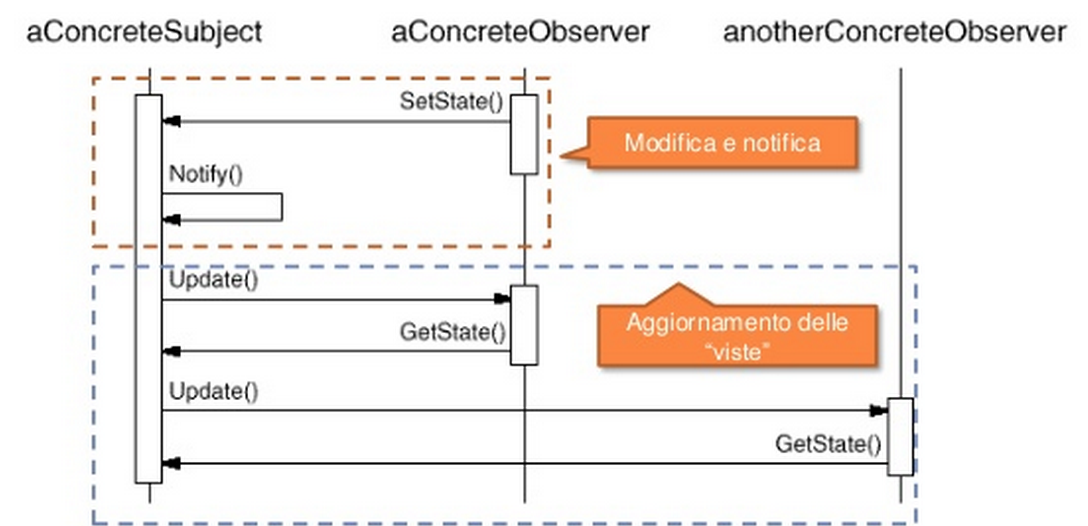
\includegraphics[width=0.8\textwidth]{immagini/observerSequence.png}
    \caption{Proxy}
\end{figure}
\FloatBarrier


\subsubsection{Casi tipici}
\begin{itemize}
\item Quando è necessario che al cambiamento di stato di un oggetto, altri oggetti eseguano delle azioni;
\item Quando è richiesto di fare il broadcast di un evento;
\item Per ottenere un accoppiamento ``astratto'' tra soggetti e osservatori.
\end{itemize}